\documentclass[master=cws,masteroption=se,english]{kulemt}
\setup{% Verwijder de "%" op de volgende lijn bij UTF-8 karakterencodering
  %inputenc=utf8,
  title={The best master's thesis ever},
  author={Ruben Kindt},
  promotor={Prof.\,dr.\ Tias Guns},
  assessor={ },
  assistant={}}
% Verwijder de "%" op de volgende lijn als je de kaft wil afdrukken
%\setup{coverpageonly}
% Verwijder de "%" op de volgende lijn als je enkel de eerste pagina's wil
% afdrukken en de rest bv. via Word aanmaken.
%\setup{frontpagesonly}

% Kies de fonts voor de gewone tekst, bv. Latin Modern
\setup{font=lm}

% Hier kun je dan nog andere pakketten laden of eigen definities voorzien
\usepackage{todonotes}

% Tenslotte wordt hyperref gebruikt voor pdf bestanden.
% Dit mag verwijderd worden voor de af te drukken versie.
\usepackage[pdfusetitle,colorlinks,plainpages=false]{hyperref}

%%%%%%%
% Om wat tekst te genereren wordt hier het lipsum pakket gebruikt.
% Bij een echte masterproef heb je dit natuurlijk nooit nodig!
\IfFileExists{lipsum.sty}%
 {\usepackage{lipsum}\setlipsumdefault{11-13}}%
 {\newcommand{\lipsum}[1][11-13]{\par Hier komt wat tekst: lipsum ##1.\par}}
%%%%%%%

%\includeonly{chap-n}
\begin{document}

\begin{preface}
  I would like to thank everybody who kept me busy the last year,
  especially my promoter and my assistants. I would also like to thank the
  jury for reading the text. My sincere gratitude also goes to my wive and
  the rest of my family.
\end{preface}


\listoftodos

\tableofcontents*

\begin{abstract}
	\todo{abstract}
  The \texttt{abstract} environment contains a more extensive overview of
  the work. But it should be limited to one page.

  \lipsum[1]
\end{abstract}

\begin{abstract*}
	\todo{samenvatting}
  In dit \texttt{abstract} environment wordt een al dan niet uitgebreide
  Nederlandse samenvatting van het werk gegeven.
  Wanneer de tekst voor een Nederlandstalige master in het Engels wordt
  geschreven, wordt hier normaal een uitgebreide samenvatting verwacht,
  bijvoorbeeld een tiental bladzijden. 

  \lipsum[1]
\end{abstract*}

% Een lijst van figuren en tabellen is optioneel
%\listoffigures
%\listoftables
% Bij een beperkt aantal figuren en tabellen gebruik je liever het volgende:
\listoffiguresandtables
% De lijst van symbolen is eveneens optioneel.
% Deze lijst moet wel manueel aangemaakt worden, bv. als volgt:
\chapter{List of Abbreviations and Symbols}
\section*{Abbreviations}
\begin{flushleft}
  \renewcommand{\arraystretch}{1.1}
  \begin{tabularx}{\textwidth}{@{}p{12mm}X@{}}
    LoG   & Laplacian-of-Gaussian \\
    MSE   & Mean Square error \\
    PSNR  & Peak Signal-to-Noise ratio \\
  \end{tabularx}
\end{flushleft}
\section*{Symbols}
\begin{flushleft}
  \renewcommand{\arraystretch}{1.1}
  \begin{tabularx}{\textwidth}{@{}p{12mm}X@{}}
  	delta-debugging
  	catigorize 
  	grammer based fuzzing
  	blackbox fuzzing
  	gray box fuzzing
  	white box fuzzing
  	hierarchical delta-debugging
  	1-minimal
  	grammar based fuzzing
  	MUS %minimal unsat subset =/= 
  	
    42    & ``The Answer to the Ultimate Question of Life, the Universe,
            and Everything'' according to \cite{h2g2} \\
    $c$   & Speed of light \\
    $E$   & Energy \\
    $m$   & Mass \\
    $\pi$ & The number pi \\
  \end{tabularx}
\end{flushleft}

% Nu begint de eigenlijke tekst
\mainmatter

\chapter{Introduction}
\label{cha:intro}
There are a lot of causes for bugs: software complexity, multiple people writing different parts, changing objective goals, misaligned assumptions and more. Most these things can not be avoided during the creation of software but are the cause of program crashes, vulnerabilities or wrong outcomes. Multiple forms of prevention have been created like: the various forms of software testing, documentation, automatic tests and code reviews. All with the aim to prevent the occurrence of bugs and to reduce the cost associated with them. While automatic test cases often evaluate the goals of software end evaluate previous known bugs, it can do much more. Fuzzing software is a part of those automatic tests, a technique that is popular in the security world for exploit prevention. This technique generates random input for a program under test (PUT) and monitors if the program crashes or not. This explanation was the original interpretation of fuzzing as preformed by Miller\cite{4originalFuzzingUnixUtils}, today this technique is seen as random generation based black box fuzzing while the current fuzzing envelops a broader term, as Man\`es et al.\cite{13manes2019survey} put it nicely,
\begin{quote}
"Fuzzing refers to a process of repeatedly running a program with generated inputs that may be syntactically or semantically malformed."
\end{quote}, as quoted from \cite{13manes2019survey}.
With this technique we will try to detect bugs in the constraint programming and modeling library CPMpy \cite{17guns2019increasing} created by Prof. dr. Guns et al.

\todo{modus operandi bij intro}

\section{The usage of fuzzers in the software development cycle}
During the development phase of software, tests are preformed to check if the written code matches the expected and wanted output. This can be done by the developers themselves or by quality assurance testers which do this full time and this on multiple different ways: code review, manual testing or automated testing. Those could exist out of unit tests, checking for known bugs, confirming that the use cases are working, code audits, dynamic testing, fuzzing and others. None of the techniques mentioned above can prevent all possible bugs from occurring on top of that using only a single technique would cost more to find the same level of bugs then using multiple techniques. Sometimes a code audit is better, for example in situations where you want to know something easy that is most likely plainly written in the code. Other cases dynamic testing may be better, image you have a program which parses curricula vitae to check if candidates match the job position and you want to check if fresh Computer science graduates match the position software analyst. In this case it may be a lot easier to simulate the use case than to dive into the code. In situations where you want to test if bugs exist, you may not know where to start inside of the PUT, this is where Fuzzing may be the correct tool to use. Fuzzing emerged in the academic literature at the start of the nineties, while the industry's full adoption thirty years later is still ongoing. Multiple companies like Google, Microsoft and LLVM have created their own fuzzers and this together with a pushing security sector for the adoption has caused fuzzing to become a part of the growing toolchain for software verification.

\section{Fuzzing and security}
The adoption of fuzzers has definitely gained speed due to its proven effectiveness in finding security exploits. For example ShellShock, Heartbleed, Log4Shell, Foreshadow and KRACK could have been found using fuzz testing as shown in multiple sources \cite{ShellShockViaFuzzing}, \cite{HeartbleedViaFuzzing}, \cite{Log4ShellViaFuzzing}, \cite{34ForeshadowViaFuzz} and fuzzing is even recommended by the authors to prevent similar exploits \cite{33KrackViaFuzz} and \cite{35ForeshadowFuzzRecom}.

\section{Constraint programming in general}
%	what is CP and family, differences, \cite{freuder1997pursuit}
%	usage
%	what could go wrong, cost of bugs

\section{CPMpy}
%	section on how CPMpy works and convorts for other solvers \cite{CP2021 Tutorial "CPMpy, a Numpy-based CP Modeling Environment} and \cite{https://github.com/CPMpy/cpmpy/} and where errors could occure, whitch ones are in/out of scope

\section{fuzzing history}
% why fuzzing, ref to securrity and \cite{25MillerOnMacOS} examples of viruese
%bit of history around fuzzing or CP
% first study in fall of 1988 paper in 1990
% miller 2020 heeft hiervoor de start aan bronnen, pagina 2 middel of linker kolomn
%	generation based, mutation based | White gray, back box | directed fuzzing, coverage-based fuzzing \cite{11Fuzzingasurvey}


%%% Local Variables: 
%%% mode: latex
%%% TeX-master: "thesis"
%%% End: 

%Ideas 
%context
%	what is CP and family, \ref{freuder1997pursuit}
%	usage
%	what could go wrong
%
%
%bit of history around fuzzing or CP?
% first study in fall of 1988 paper in 1990
% miller 2020 heeft hiervoor de start aan bronnen, pagina 2 middel of linker kolomn
%
%Chapter about (psuedo-)randomness
%
%chapeter on simplifying the crashes
%	binary search will not work all the time
%	quarters remove may work (if all parts fail go more granular, 1/9 or 1/16)
%		start with halfs then *2
%		always search further with same granularity but with removed part until all options with that granularity searched \ref{zeller2009programs} p111
%		this uses no knowledge from input structure and program structure \ref{zeller2009programs} p112
%	delta debugging
%		time spend searching vs simplified ratio is important as mentioned in \ref{mansur2020detecting}
%		and needs to preserve satisfiability as mentioned in \ref{mansur2020detecting}
%		^ possibly a big deal to find critical bugs
%
%	with knowadge of input, syntax \ref{zeller2009programs}
%	of by bigger entities like lines of words \ref{zeller2009programs}
%	 for speed
%
%	alt approach like \ref{mansur2020detecting} try finding the bug again with less resources avail
%	or isolaytion \ref{zeller2009programs} p 285 
%		I think it may fail if multiple parts are relevant
%		I think it could detect for example the CPMpy import as a bug cause as the min diff that causes the bug
%
%	sub section on MUS/minimum unsat subset vs delta debugging
%		MUs good for only whole constraints while 
%		delta debugging goes for partial structures
%
%	section on how CPMpy works and convorts for other solvers \ref{CP2021 Tutorial "CPMpy, a Numpy-based CP Modeling Environment} and \ref{https://github.com/CPMpy/cpmpy/} and where errors could occure, whitch ones are in/out of scope
%
%
%	isolation vs simplifying \ref{zeller2009programs} p 285
%
%
%avoiding inf loops -> timeouts
%The Precision Effect minimizing/simplyfying may lead to a dif found bug if multiple, since all need to be solved not problem  \ref{zeller2002simplifying}
%	 can be sloved with stack trace comparison
%
%section on minimalisation vs isolation \ref{zeller2002simplifying} p12
%	for speed take smaller inputs
%	Isolation will require a lot more things to track but is faster
%	
%Chapter around fuzzing
%	\ref{mathis2019parser} states 3 optins traditional, stochastic and syntax driven.
%
%chapter results
%chapter comparison to other fuzzers
%

\chapter{The First Chapter}
\label{cha:1}
A chapter is a logical unit. It normally starts with an introduction, which
you are reading now. The last topic of the chapter holds the conclusion.

\section{The First Topic of the Chapter}
First comes the introduction to this topic.

\lipsum[55]

\subsection{An item}
Please don't abuse enumerations: short enumerations shouldn't use
``\verb|itemize|'' or ``\texttt{enumerate}'' environments.
So \emph{never write}: 
\begin{quote}
  The Eiffel tower has three floors:
  \begin{itemize}
  \item the first one;
  \item the second one;
  \item the third one.
  \end{itemize}
\end{quote}
But write:
\begin{quote}
  The Eiffel tower has three floors: the first one, the second one, and the
  third one.
\end{quote}

\section{A Second Topic}
\lipsum[64]

\subsection{Another item}
\lipsum[56-57]

\section{Conclusion}
The final section of the chapter gives an overview of the important results
of this chapter. This implies that the introductory chapter and the
concluding chapter don't need a conclusion.

\lipsum[66]

%%% Local Variables: 
%%% mode: latex
%%% TeX-master: "thesis"
%%% End: 

\chapter{Fuzzing}
\label{cha:2:fuzzing}
\label{cha:2:intro}
The rise of fuzzing came with Miller giving a classroom assignment\cite{21FuzzingAssignment} in 1988 to his computer science students to test Unix utilities with randomly generated inputs with the goal to break the utilities. Two years later in December he wrote a paper\cite{4originalFuzzingUnixUtils} about the remarkable results, that more than 24\% to 33\% of the programs tested crashed.
In the last thirty years the technique of fuzzing has changed significantly and various innovations have come forward. In this chapter we will look at classifications made, what the fuzzer expects as input, what we can expect as output and we will look at the most popular fuzzers.

\section{Classifications}
\label{cha:2:Classifications}
The three most popular classifications are\cite{12Fuzzingasurvey}\cite{13manes2019survey}\cite{30FuzzingHackartandscience}: how does the fuzzer create input, how well is the input structured and does the fuzzer have knowledge of the program under test (PUT)?

\subsection{Generation and mutation}
\label{cha:2:generationMutation}
A fuzzer can construct inputs for a PUT in two ways, it can generate input itself or it can take an existing input, called seeds, and modify them. While Generation is more common when it comes to smaller inputs, the opposite is true for larger inputs where modification has the upper hand. This is cause by the fact that generating semi-valid input becomes a lot harder the longer the input becomes. For example, generating the word "Fuzzing" by uniformly random sampling ASCII, has a chance of one in $5*10^{14}$ of happening, making this technique infeasible when we want to generate bigger semi-valid inputs. With mutation we can start with larger and already valid input and make modifications to create semi-valid inputs. With this last technique the diversity of the seeding inputs does become quite important. Ideally we would have an unlimited diverse set of inputs, but due to limited computation and available inputs we sometimes need to take a subset. In a paper by Alexandre Rebert et al. \cite{14rebert2014seedselecting} they propose that seed selection algorithms can improve results and compare random seed selection to the minimal subset of seeds with the highest code coverage among other algorithms. 

\subsection{Input structure}
\label{cha:2:InputStructure}
%lexical, sementical, constraint or random
While we have discussed the bigger scope on how inputs are created, let us go into more detail; as we have seen before, fuzzing started with Miller's classroom assignment. This random generation of inputs falls under 'dumb' fuzzing due to only seeing the input as one long list of independent symbols with no knowledge of any structure. This technique can be applied similarly to mutational fuzzing as well, compared to only adding symbols with generational fuzzing here we also remove or change randomly selected symbols. 
We can create three types of inputs: non-valid semi-valid and valid inputs. With non-valid inputs we will almost be exclusively testing the syntactic stage of the PUT, often called the parser. Either the input crashes the parser or it will be detected as invalid by the parser and the PUT will stop running. With semi-valid inputs we hope to be as close as possible to valid inputs in order to explore beyond the parser and to catch bugs deeper in the PUT. And lastly with valid input we are testing if the PUT behaves as expected and does not crashes.
A smarter technique is referred to techniques, which have knowledge about the structure inputs can or should have. This increases the chance of inputs passing the parser and being able to test the deeper parts of the PUT, this at the cost of needing an increased complex fuzzer. We can build a 'smart' fuzzer by adding knowledge about keywords (making it a lexical fuzzer) or by adding knowledge about syntax (for a syntactical fuzzer, which can for example match all parentheses). Directed fuzz testing, where we guide the fuzzer on a specific path, does fit in this category of a 'smart' fuzzer as well but it is not possible in a black box environment, more on that in the next section.

\subsection{Black, gray and white box fuzzing}
\label{cha:2:BlackGrayWhiteFuzzing}
Now that we have discussed adding knowledge of inputs to the fuzzer, we can also add knowledge about the PUT to the fuzzer. Which brings us to black, gray and white box fuzzing. With black box fuzzing we have no knowledge about the inner working of the PUT and we treat the PUT as a literal black box, we provide input and we look at what comes out. With this minimal information the fuzzer then tries to improve its input creation. Compared to black box fuzzing, gray box fuzzing usually comes with tools that give indirect information to the fuzzer. Tools like: code coverage, timings, classes of errors as measurements are all used as feedback, but more measurements are possible. Lastly, as you may have predicted, white box testing is the term used when the fuzzer has as much information to it available as possible. It will have access to the source code and can adjust their inputs to fuzz specific parts of the code (this falls under directed fuzzing). White box fuzzing does have a higher computation cost due to having to reverse engineer the path to specific edge cases, meaning that it can find more bugs per input but creating those inputs takes more time compared to black box fuzzing. The differentiation between black, gray and white box fuzzing is not clear cut, most people would agree that white box fuzzing has full knowledge about the PUT, including the source code, that gray box fuzzing has some knowledge about the PUT and that black box fuzzing has little to no knowledge about the PUT. Going into more detail, all we can say is that it is no longer a black-and-white situation and that the lines has become fuzzy. \todo{Ask permission to do this}

\section{Classifying fuzzers}
\label{cha:2:OtherFuzzers}
Now that we know how we can classify fuzzers, let us look at some existing fuzzers to see how they work. For starters Miller's original work, which we discussed earlier, was a random generation based black box fuzzing. And started off as an assignment for his students to test the reliability of Unix utility programs by trying to break them using a fuzz generator, which was able to generate printable ASCII, non-printable ASCII, with or without null terminating characters of a random length. That resulted in a successful paper\cite{4originalFuzzingUnixUtils} two years later. His later work in 1995 on even more UNIX utilities, his work on X-Windows servers\cite{26miller1995fuzzrevisited}, his work in 2000 on Windows NT 4.0 and Windows 2000\cite{24MillerWindows}, his work on MacOS\cite{25MillerOnMacOS} and his later revisit\cite{3miller2020relevanceOfClasicalFuzzTesting} on fuzzing all fall in the same category of random generation based black box fuzzing. This papers showed that a significant portion of programs are able to be crashed with random inputs. Of the programs tested 15 to 43\% of the Unix utilities crashed, 6\% of the open-source GNU utilities crashed, 26\% of X-Window applications crashed, 45\% of Windows NT 4.0 and Windows 2000 programs crashed and 16\% MacOS programs crashed.

A couple of years later, KLEE\cite{8KLEE} was developed by Cadar et al. KLEE is a generation based white box fuzzing tool build with the idea that bugs could be on any code path and that testing should cover as code much as possible. A code coverage tool is used to test which lines of code are executed and this combined with the feedback KLEE got from the symbolic processor and the interpreter it can generate improved inputs. KLEE does this by symbolically executing the program executions branching on any dangerous operations and when it finds an error it will convert the symbolic to a concrete representation based on the constraints it needed to get passed the specific branches and uses this concrete representation to test the original program.With this stride to obtain 100\% code coverage it should be noted that covering a line of code does not mean that line of code has been found to contain no bugs, but not going over lines of code definitely means that the lines remain untested. Therefore code coverage code coverage is sometimes used as a relative metric, checking if a specific test raises the code coverage, means that a test uses a new part of the code base that has not been tested yet. This combined with the fact that getting a high code coverage is a demanding task and does not easily gets to 100\% turns code coverage into a well rounded measurement.

As for the more popular fuzzers, is the American fuzzy lop\footnote{\url{https://github.com/google/AFL}} (AFL), which named after a rabbit breed and is a C and C++ focused mutation based gray box fuzzer released by Google. But due inactivity on Google's part the fork AFL++\footnote{\url{https://github.com/AFLplusplus/AFLplusplus}} has become more popular than the original and is maintained actively by the community\cite{27AFL++}. Not only is it actively maintained, it is also actively used by researchers like: Lennert Wouters who used it to extract SpaceX Startlinks user terminal firmware \footnote{\url{https://www.esat.kuleuven.be/cosic/blog/dumping-and-extracting-the-spacex-starlink-user-terminal-firmware/}}. \todo{watch his talk, read paper}
Not only did AFL spark AFL++, it has also sparked a python\footnote{\url{https://github.com/jwilk/python-afl}} focused version, a Ruby\footnote{\url{https://github.com/richo/afl-ruby}} focused one, a Go\footnote{\url{https://github.com/aflgo/aflgo}} focused version and is shown by Robert Heaton\cite{AFLWrapper} to not be difficult to write a wrapper for it. 

A potential reason to the inactivity of Google on the ALF project could be the development of both Clusterfuzz\footnote{\url{https://google.github.io/clusterfuzz/}} and OSS-fuzz\footnote{\url{https://google.github.io/oss-fuzz/}}, a scalable fuzzing infrastructure and a combination of multiple fuzzers respectively. With the former one being used in OSS-fuzz as a back end to create a distributed execution environment. This with quite a bit of success\cite{31OSS-FuzzBugs},
\begin{quote} \todo{September update this}
	"As of July 2022, OSS-Fuzz has found over 40,500 bugs in 650 open source projects.",
\end{quote} according to the repository itself. 
Not only Google has come forward with a fuzzer. Even Microsoft has jumped on board of fuzzing with OneFuzz\footnote{\url{https://github.com/microsoft/onefuzz}}, a self-hosted Fuzzing-As-A-Service platform which is intended to be integrated with the CI/CD pipeline. Although looking at the given stars on the Github repository, it looks like Google's tools are more popular than Microsoft' ones.
The last prominent fuzzer we are going to take a look at is the LibFuzzer\footnote{\url{https://llvm.org/docs/LibFuzzer.html}} made by LLVM, a generation based gray box fuzzer which is a part of the bigger LLVM project\footnote{\url{https://github.com/llvm/llvm-project/}} with the focus on the C ecosystem. Being in the same ecosystem as AFL, LibFuzzer can be used together with AFL and even share the same seed inputs.

\subsection{Testing CP and SMT with Fuzzers}
Until now we discussed fuzzers more generally, we would like to deliberate specific fuzzers build for testing constraint programming languages (CP) and satisfiability modulo theory (SMT) solvers.


\begin{figure}
	\centering
	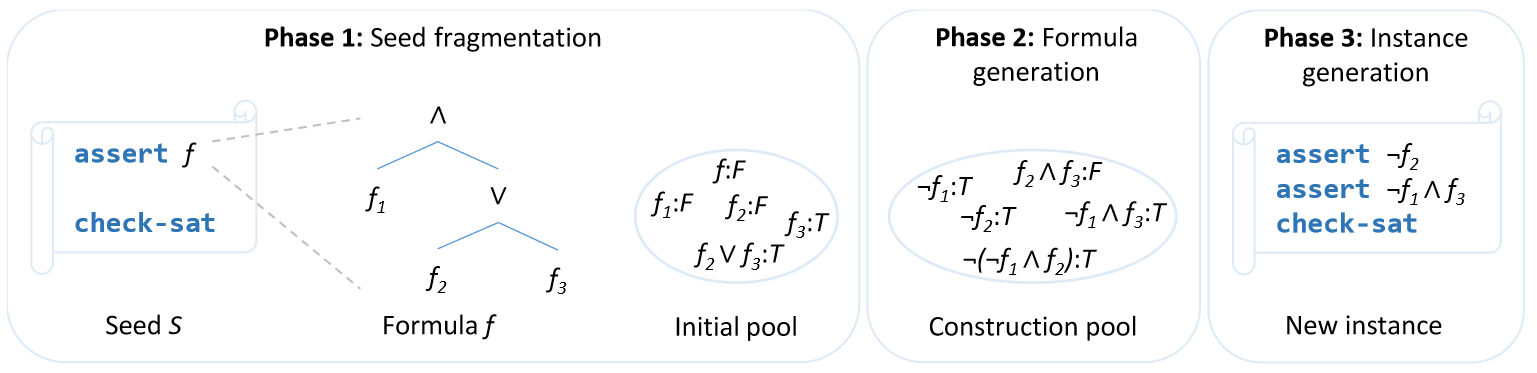
\includegraphics[width=1.0\textwidth]{images/STORM}
	\caption{Overview of the three STORM phases as presented by Muhammad Numair Mansur et al. in "Detecting Critical Bugs in SMT Solvers Using Blackbox Mutational Fuzzing"\cite{1mansur2020detecting}.}
	\label{fig:STORM}
\end{figure}
One of those fuzzers is STORM which is a mutation based black box fuzzer created by Muhammad Numair Mansur et al.\cite{1mansur2020detecting} to find critical bugs in SMT solvers. In their paper they explain the inner working thoroughly, but briefly summarized STORM creates an initial pool of smaller formulas from  existing formulas found in seeds, uses another solver to create models of those smaller formulas. To then construct more complex formulas with the knowledge of their ground truth, with this STORM can test the SMT solver as can be seen in figure \ref{fig:STORM}. This novel way of fuzzing SMT solvers with inputs that are satisfiable by construction and has been cited significantly considering that it is a recent paper.


Another technique for fuzzing SMT solvers is the one proposed by Dominik Winterer et al. with their fuzzer YinYang\cite{43YinYang}, which uses "Semantic Fusion" to test the solvers.
\begin{quote}
	"Our key idea is to fuse two existing equisatisfiable (i.e., both satisfiable or unsatisfiable) formulas into a new formula that combines the structures of its ancestors in a novel manner and preserves the satisfiability by construction. This fused formula is then used for validating SMT solvers."
\end{quote} As quoted from "Validating SMT Solvers via Semantic Fusion"\cite{43YinYang}
Dominik Winterer et al. take a free variable from each of the equisatisfiable formulas to be able to create a new variable using a reversible fusion function. For example a formula $\phi_1$ = X > 10, $\phi_2$ = Y < 9 with the fusion function for Z = X + Y would become $\phi_3$ = Z - Y > 10 $\land$ Z - X < 9, linking both satisfiable formulas together. For unsatisfiable formulas an extra conjunction is needed with the definition of the new variable, because a substitution could result in the loss of the unsatisfiability of the formula as mentioned in the paper. The results of the paper where also significant with 45 bugs in state-of-the-art SMT solvers in Z3\footnote{\url{https://github.com/Z3Prover/z3}} and CVC4\footnote{\url{https://cvc4.github.io/}}. Dominik Winterer et al. also give multiple fusion functions like multiplication and string concatenations which can be applied to integers and real numbers and strings respectively. Extending this technique to other data types or more fusion functions would not be difficult.

\todo{falcon} paper 42 fits well here


\subsection{Types of bugs}
\todo{add different result both say sat but One says 'X=9' other says x="10"}
\label{cha:2:TypesOfBugs}
We can also classify the types of bugs found by the fuzzers, as done in a recent paper\cite{1mansur2020detecting} by Muhammad Numair Mansur et al. being: crashes, wrongly satisfied, wrongly unsatisfied or a hanging PUT. With some of these bugs being less acceptable then others. For example, as Muhammad Numair Mansur et al. describes, a crash is preferred for a constraint programming language (CP) over a wrongly unsatisfied model, since there is no way for the user to know that the solver failed in that last case (except for differentiation testing, more on that later). Meaning that the user will treat the result (wrongly) as correct, compare this to a crash were it is clear that something went wrong. With hanging PUT's the user can not draw incorrect conclusions and with wrongly satisfied models the user can check the model's instances and confirm the result before using it further. This is due to the fact that problems are frequently np-hard meaning they are easy to confirm but hard to solve. For practical reasons we will later change the undecidable and hanging PUT's into timeouts. We know that the types of bugs can be classified in more detail, for example crashes into buffer overflows, invalid memory addressing and so on, but we choose to stay with a more general overview for now. An interesting classification to be added is the knowledge whether or not the bug is in the parser part of the PUT or not. The put could already fail on inputs during the interpretation of the inputs and as discussed we would also like to detect bugs deeper in the PUT. As the authors of "Semantic Fuzzing with Zest"\cite{22SemanticFuzzing} would classify, is the bug in the syntactical or in the semantical part of the program?

\section{The oracle problem}
\label{cha:2:OracleProblem}
% see holy grail
%\cite{11freuder1997pursuitHolyGrail}
\todo{ above thing}
%differential testing with whom? diff on what nr outputs, solutions, hash
%knowing the ground truth (STORM bin and YinYang algeb)
GT = Sat, solver = unsat vs GT = unsat solver = sat

The oracle problem describes the issue of telling if a PUT's output was, given the input, correct or not or as said in "The Oracle Problem in Software Testing: A Survey"\cite{10barr2014oracleProblem} 
\begin{quote}
	"Given an input for a system, the challenge of distinguishing the corresponding desired, correct behavior from potentially incorrect behavior is called the test oracle problem."
\end{quote} by Barr et al.
In their paper they discuss four categories: specified test oracles, derived test oracles, implicit test oracles and the absence of test oracles. The biggest category would be the specified test oracles which contains all the possible encoding of specifications like: modeling languages UML, Event-B and more. Their derived test oracles classification contains all forms of knowledge obtained from documentation on how the program should work or by knowledge of previous versions of the program. The last two oracles categories come down to the use of knowing that crashes are always unwanted and the human oracle like crowdsourcing respectively.

\subsection{Handling the oracle problem}
\label{cha:2:handelingOracelproblem}
Although the approach of by Bugariu and M\"uller in "Automatically testing string solvers"\cite{9bugariu2020automaticallyTestingStringSolvers} falls in the first category mentioned above, their approach is innovative. While most fuzzers either use crashes or differential testing (more on that later) to find bugs, they know the (un)satisfiability of their formulas by the way of they are constructed. For satisfiable formulas they generate trivial formulas and then by satisfiability preserving transformations increase the complexity and for unsatisfiable formulas they use $\neg$ A $\land$ A', with A' being a equivalent formula of A, to create the trivial unsatisfiable formulas. To increase the complexity of those trivial formulas, they again depend on satisfiability preserving transformation. This technique of creating formulas satisfiable by construction has also been applied to SMT solvers by Muhammad Numair Mansur et al. called STORM\cite{1mansur2020detecting} which uses mutational input creation compared to the previous generation based techniques. In the paper the authors dissect all SMT assertions into their sub-formulas and create an initial pool. In this pool the sub-formulas are checked if they satisfy or not and with this knowledge new formulas are created for the population pool with ground truth, from this pool new theories are created and tested. This makes that STORM does not need an oracle to test the entire theory, but only the smaller sub-formulas.
%deze controleert dat de sat is still valid by using another solver as oracle (bij het annoteren van T/F values in the init pool)
% de eerste gebruikt een oracle bij het controleren of dat de equi transformations het model niet breken

\subsection{Differential testing}
\label{cha:2:Differential}
As mentioned above a lot of fuzzers use crashes to detect that the PUT has failed to provide a correct output or when possible use differential testing. This latter one uses a single or multiple analogue programs to test if the PUT gave the same output as the analogue programs. Neither techniques is complete: crash based fuzzing can not detect wrong outputs and differential testing requires that one or multiple analogue programs exits and each with an different implementation to get no overlapping bugs. The latter technique may therefore not always be possible due to the existence of those analogue programs.
\todo{ metamorphic testing}

%somewhere a ref to later chapter input simplification (minimisation differantioation)
\todo{this section}
\section{Opinions against Fuzzing}
\label{cha:2:againstFuzzing}
Unreasonable, why would a person do this, creates unnecessary more work to fix
\cite{39differentialTesting} although has focus on diff testing
this fits well with the types of bugs and with other toolchain
although we have a bias due to writing a dissertation about fuzzing, we think that WE are correct and THEY are wrong, proofs see above + finding bugs/exploits is important

\section{Conclusion}
\label{cha:2:conclusion}
\todo{conclusion}
The final section of the chapter gives an overview of the important results
of this chapter. This implies that the introductory chapter and the
concluding chapter don't need a conclusion.


%%% Local Variables: 
%%% mode: latex
%%% TeX-master: "thesis"
%%% End: 

\chapter{Detecting crucial parts in inputs}
\label{inputReduction:intro}
When we detect that the program under test (PUT) crashes, wrongly satisfies, wrongly unsatisfies, hangs or gives the wrong solution on a given input we want to know why it does that. What causes this unwanted output and on what line does the bug occurs. With crashes, a stack trace and some luck this could be easy, but when a bug causes a crash in another place or we get another unwanted output the developer may need to debug deep into the code to find the bug. This with a potential large inputs could be a tedious and long assignment, for this reason we would like to know what parts of the input are relevant for the bug. We will discover this further in this chapter, starting with deobfuscating inputs.

\todo{cont here}
\section{Deobfuscating inputs}
\label{inputReduction:Deobfuscating}
\begin{quote}
	"Often people who encounter a bug spend a lot of time investigating which changes to the input file will make the bug go away and which changes will not affect it." 
	\newline
	-Richard Stallman and Ralf Hildebrandt in "Simplifying and Isolating Failure-Inducing Input" \cite{5zeller2002simplifyingIsolatingFailure-inducing}.
\end{quote} 
When receiving a big input the chance of it having parts unrelated to the bug is almost guaranteed, we will call these inputs (unintentionally) obfuscated inputs. Deobfuscating those inputs can take a lot of try and error to see which variations still reveal the bugs or having to walk through the execution to find the bugs. Both take a while if we want to go to absolute minimal inputs, but for developers it is not needed to go to that extreme. As long as we take the bulk of the unrelated parts of inputs away it will help the developer to find the bug faster. With these techniques we can also group similar bugs and duplicate errors (more on that later) which is also fairly useful information for developers.
\subsection{Simplifying}
\label{inputReduction:Simplifying}
To find crucial parts of inputs, it is often achieved either with simplification or Isolation. 
Simplification is the technique where we repeatably remove parts of a failing input and check if it still fails and it often called "delta-debugging", which belongs to the divide-and-conquer family of algorithms \cite{2FuzzingAndDeltaDebuggingSMTSolvers}. 
The algorithm can be seen in figure \ref{fig:ddmin} with 
"$ c_{\mbox{\ding{56}}} $"  %c_X
meaning the failing input to be deobfuscated,
"\ding{52}" %checkmark 
meaning that a test passed with the given input,
"\ding{56}" %cross 
failed with the given input, 
"$\Delta$" and "$\nabla$" being a subset of the input and the complement of the former and
"1-minimal" meaning that not a single character can can change without the input going from failing to passing. Firstly we start the algorithm with the input and a split (n) of two. If there is a subset that still fails on it own, then we continue with that subset else we look for a subset where the complement of the input still fails but where a subsets is missing from the input. In the case where we split the input in two parts this would be the same as te previous. In case we do not find any smaller subset to continue on, then we reduce de granularity of the split by two. To finally when it is no longer possible to remove any part of the input we have obtained an input where all parts are necessary to expose the bug. This input is at the same time also the shortest possible input to trigger this bug, making finding the bug for the developer easier than in the original input filled with unrelated parts. 
An example of delta-debugging to minimize input can be found in figure \ref{fig:ddminExample}. In the first two steps no removal of any part nor complement was possible therefore we reduces the granularity, after which a removal of parts 3 and 4 was found possible. To then use some previous knowledge (lines 9, 10 and 11) with 2 new tests to remove parts 5 and 6). To then decrease the granularity again until we reach a minimal input.

\begin{figure}
	\centering
	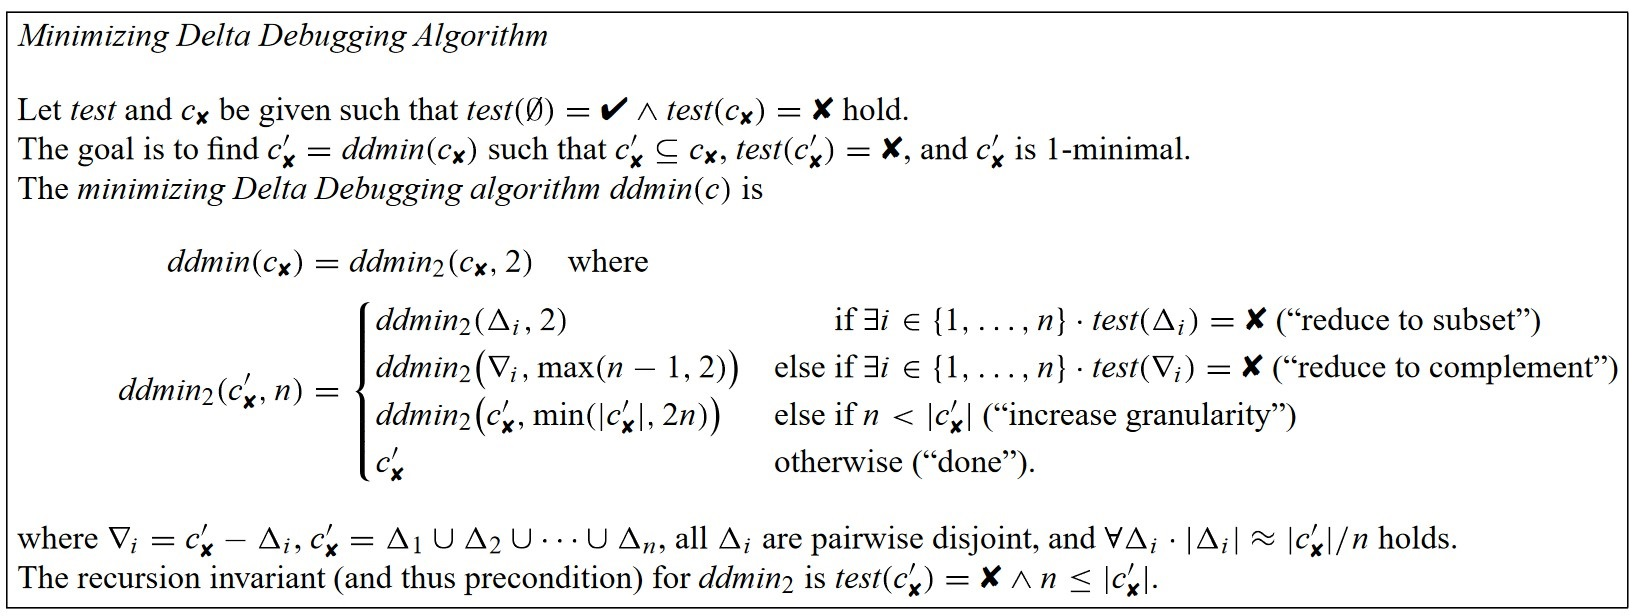
\includegraphics[width=1.0\textwidth]{images/ddminFromPaper5edit}
	\caption{A minimizing delta-debugging algorithm as shown in \cite{5zeller2002simplifyingIsolatingFailure-inducing}.}
	\label{fig:ddmin}
\end{figure}

\begin{figure}
	\centering
	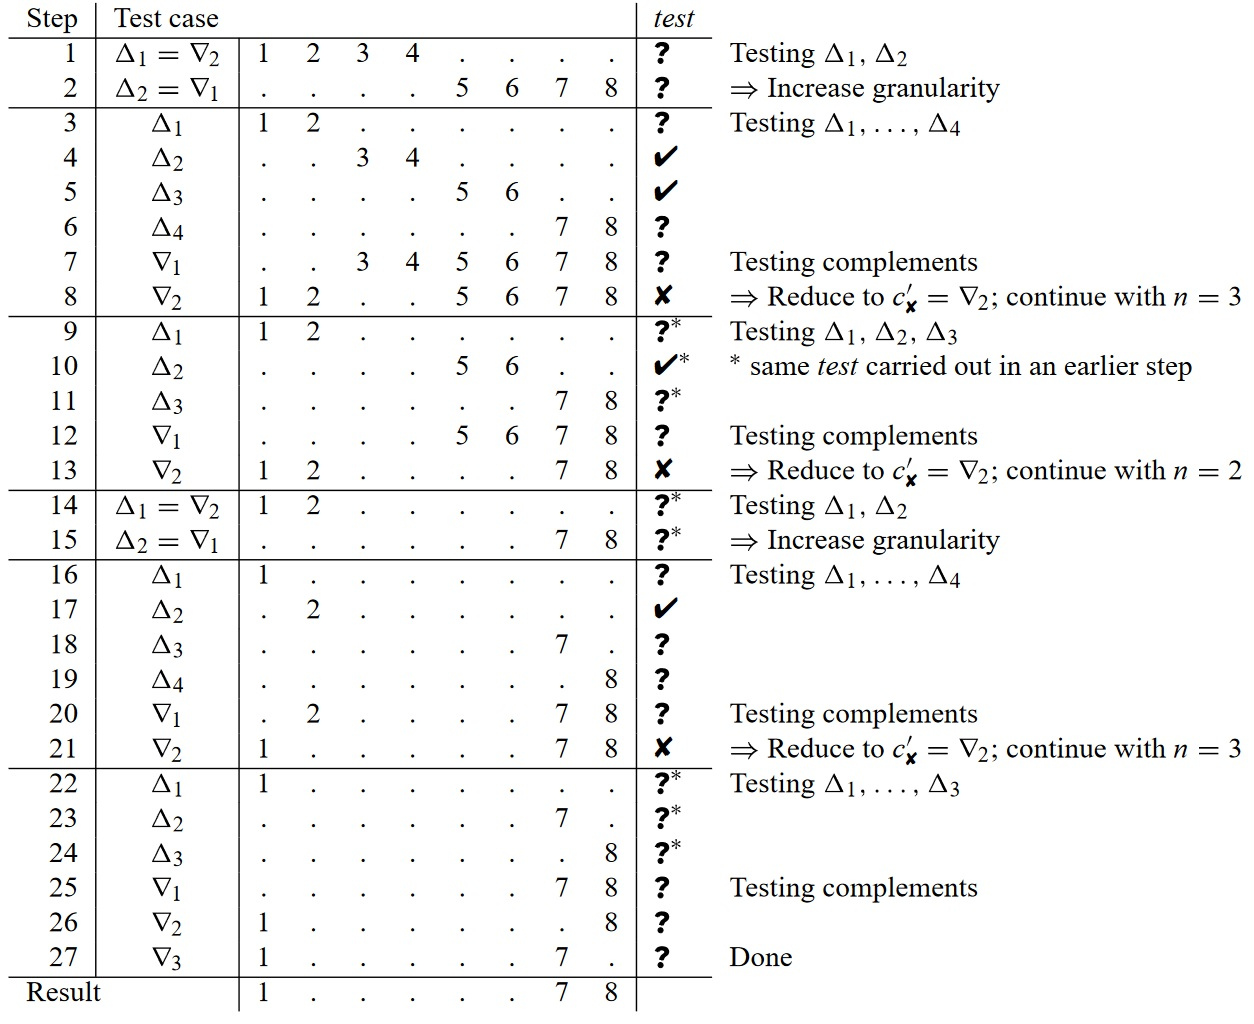
\includegraphics[width=1.0\textwidth]{images/ddminExampleFromPaper5}
	\caption{A minimizing delta-debugging example as shown in \cite{5zeller2002simplifyingIsolatingFailure-inducing} with an input that is deobfuscated with the ddmin() algorithm\ref{fig:ddmin}.}
	\label{fig:ddminExample}
\end{figure}

\subsection{Isolation}
\label{inputReduction:Isolation}
The second technique, isolation, is a technique where instead of minimizing the input we try to find the smallest difference between an input that shows the bug versus an input that does not show the bug. This with the advantage that no matter if we find the bug or not the difference will diminish, either the maximum input will shrink or the minimum input will grow. 
This technique brings extra complexity with the tracking of multiple inputs and bigger inputs often take longer, but according to Andreas Zeller et al. \cite{5zeller2002simplifyingIsolatingFailure-inducing} this is the faster one to the two techniques. 
Figure \ref{fig:simplificationIsolation} shows the difference between simplifying and isolation both finding the critical part of the input. With simplification the critical part is indicated by the last test in the figure while with isolation it is the difference of the last passed and last failed tests.
\begin{figure}
	\centering
	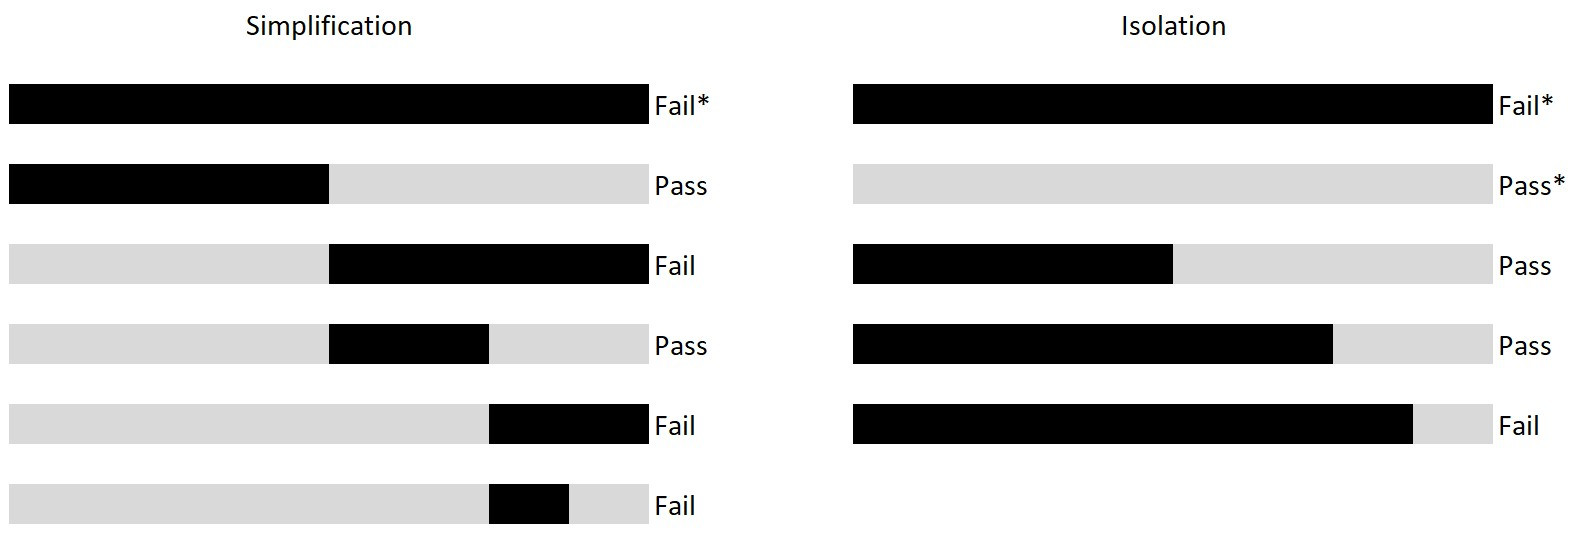
\includegraphics[width=1.0\textwidth]{images/simplificationIsolation}
	\caption{Deobfuscating inputs based on simplification (left) and isolation (right) on the same input. The '*' indicates that the result is already known and does not need to be recalculated. Figure based on an illustrations found in Why programs fail: a guide to systematic debugging by Andreas Zeller \cite{bookZellerwhyProgramsFail}.}
	\label{fig:simplificationIsolation}
\end{figure}

\subsection{Connection with minimal unsatisfiable subset and maximally satisfiable subsets}
\label{inputReduction:MUS/MSS}
For readers that are familiar with the SMT of constraint solving-world will have noticed that this techniques feels similar to a way of finding the minimal unsatisfiable subset (MUS), which it is in the case of a solver (wrongly) stating that an input is unsatisfiable. With MUS you try to find the smallest subset of formulas (or constraints) that will result in an unsatisfiable solution while with MSS you would be trying to find the biggest set of formulas (or constraints) that would result in a satisfiable solution. Both are an iterative process and can be applied in the simplification and the isolation process. But solving which combination of formulas results in the smallest of biggest subset is an computationally intensive progress. Fortunately a lot ot though has already been put in it to reduce it, for example Mark H. Liffiton et al. have proposed multiple "Algorithms for Computing Minimal Unsatisfiable Subsets of Constraints" \cite{51liffiton2008algorithms}. Again we should note that an Minimal input is not needed as we aim to reduces de input to help de developer find the error faster, a difference between a smaller and the absolute minimum will cause for a big difference in practice.

\subsection{Alternative approach}
\label{inputReduction:alt2deobfuscating}
An alternative approach compared to the already mentioned techniques is one by Alexandra Bugariu and Peter M\"uller \cite{9bugariu2020automaticallyTestingStringSolvers} is to forgo the need of deobfuscating inputs by generating inputs "small by construction". Because the smaller the inputs are the space there is for remaining stuff to obfuscate the Input. On the other hand the chance of finding bigger bugs with multiple constraints interacting with each other will be harder to find.
A last alternative approach would be retrying fuzzing by adding an increasing size limitation to find the same bug input as done by Muhammad Numair Mansur et al \cite{1mansur2020detecting}.

\section{What size to change}
\label{inputReduction:Chucksize}
A subject we glossed over is the chuck size, the size to remove while trying to find the critical parts of the inputs. 
The previous seen techniques will work well on the original fuzz testing by Miller et al. \cite{4originalFuzzingUnixUtils} since those random generated symbols where independent from each other. But when testing more complex words like function names we no longer can split on all possible places, since the input would most likely no longer parse. 
In figure \ref{fig:simplificationIsolation} we conveniently took one-eighth of the input as the chuck sizes for the ease of the example. For performance reasons we hope we can keep our chuck sizes as big as possible to be able to discard larger unrelated parts of the inputs. But when this is not possible we will need to decrease the granularity of the chuck sizes.
For example, to be able to find the critical parts of an input of the form "XXooXooXXoo" (with 'o' being the critical parts and the 'X' being unrelated to the bug) we should always search further with same granularity while the removed parts are already removed until all options with that granularity are searched \cite{bookZellerwhyProgramsFail}. This will make sure that we eliminate all unrelated parts with the specific granularity and get "ooXoooo" instead of "ooXooXXoo". 

For more complex inputs we can apply techniques seen in section \ref{fuzzing:InputStructure} where we discussed the creation of randomly and smarter created inputs. Instead of removing (hopefully) unrelated parts based purely on where the part sits in the input, we can use knowledge of the input structure or knowledge of the PUT to guide us in the removal \cite{bookZellerwhyProgramsFail}. Both lexical (the meaning of words) and syntactical knowledge (the meaning of combinations of words) can be used to help us in deobfuscating complex inputs. Where syntactical knowledge would help us remove the most since it is the bigger of the two.

\subsection{Preserving satisfiability}
\label{inputReduction:preservingSat}
With the techniques as mentioned in section \ref{cha:2:handelingOracelproblem}, "satisfiable by construction" formed inputs will need to take the extra complexity of preserving the ground truth in mind when deobfuscating inputs. When the ground truth says that an input should be unsat and the PUT says it is a satisfiable problem with the following output, then we can not remove constraints to retest if that specific constraint was the cause without knowing the new ground truth. As potential change, this could switch the original input from an unsatisfiable to a satisfiable problem. We could use a trusted solver to make sure that we only retest unsat inputs by retesting each change. or as done by  Muhammad Numair Mansur et al.'s \cite{1mansur2020detecting} technique of trying to fuzz the same seed in the hope to find a smaller input that gives the same bug. Or use other SMT solvers to make sure that the ground truth does not change as Brummayer and Biere \cite{2FuzzingAndDeltaDebuggingSMTSolvers} did.
In the other scenario when he ground truth says that an input should be sat with X amount of models and the PUT says that the input is unsatisfiable. Then we have more options to deobfuscate the inputs. We can use the previously mentioned techniques like the other scenario but we can also use simplifying, isolation, MUS, MSS and the technique of refuzzing like STORM while still preserving the (un)satisfiability of the problem.

\section{The precision effect}
\label{inputReduction:PersisionEffect}
This finding of the same bug needs to be done carefully, so that we do not change a null pointer dereference bug to a parser related bug. This, as discussed in the previous chapter, is because we value some bugs with more importance than others. 
In a paper by Andreas Zeller and Ralf Hildebrandt \cite{5zeller2002simplifyingIsolatingFailure-inducing} they talk about this exact problem which they called "the Precision Effect". Sometimes this is not a problem, for example when we are trying to find all possible bugs and will rerun the fuzzer after each incremental improvement or the situation where a deeper bug turns into another deep bug. But overall we try to avoid this effect, which can be done with the techniques in the following section.

\section{Deduplication}
\label{inputReduction:Deduplication}
With deobfuscating the inputs we can detect exact copies, but depending on the deobfuscation's time complexity other techniques could be better with similar results. In case where we would have access to stack traces (via crashes) we could differentiate the bugs on the basis of the hash from the backtrace, sometimes even numerous hashes per input depending on the amount of backtrace lines taken. This technique is called "stack backtrace hashing" and is quite popular according to Valentin J.M. Man\`es et al. \cite{13manes2019survey} 
Another technique talked about in that paper, is looking at the code coverage generated by the inputs where the executed path (or hash of it) is used as a fingerprint of the inputs. A technique, used by Microsoft \cite{36semanticsAwareDeduplicationRETracer} is called "semantics based deduplication", where instead of backtrace they use memory dumps to hopefully find the origins of bugs. This use of dumps is less ideal due to traces having more information, but the latter is not always possible due to the performance overhead and privacy causes as specified in the paper. 
A last technique would be looking at the bug description left by manual bug reports, although this dependence on the quality of bug reports and is most likely poorly automatable. 
None of the techniques mentioned above are perfect: with stack backtrace hashing you need access to the backtrace, with coverage some inputs will generate extra function calls and the semantics based deduplication are limited to X86 or x86-64 code with the binary file and the debug information. Neither of those first techniques will work with black box fuzzing unfortunately.

\section{Conclusion}
\label{inputReduction:Conclusion}
In this chapter we discussed why a reduced failing input would be convenient for the further process, what advantages it brings with it while fuzzing PUTs. We have seen multiple methods of deobfuscating inputs from the straightforward simplifying to the heavier isolation. We also looked at state of the art approaches, how they preserve satisfiability and how to avoid having to deobfuscate inputs in the first place. To then end with the advantage of short deobfuscated inputs to prevent duplicates bugs.

%%% Local Variables: 
%%% mode: latex
%%% TeX-master: "thesis"
%%% End: 

\chapter{Result}
\label{cha:4}
\todo{intro ch 4}

% own results 
% comparision with other fuzzers

\section{The First Topic of this Chapter}
\lipsum[78]


\section{Figures}
Figures are used to add illustrations to the text. The \fref{fig:logo} shows
the KU~Leuven logo as an illustration.
\begin{figure}
	\centering
	
\includegraphics{logokul}
	\caption{The KU~Leuven logo.}
	\label{fig:logo}
\end{figure}

\section{Tables}
Tables are used to present data neatly arranged. A table is normally
not a spreadsheet! Compare \tref{tab:wrong} en \tref{tab:ok}: which table do
you prefer?

\begin{table}
	\centering
	\begin{tabular}{||l|lr||} \hline
		gnats     & gram      & \$13.65 \\ \cline{2-3}
		& each      & .01 \\ \hline
		gnu       & stuffed   & 92.50 \\ \cline{1-1} \cline{3-3}
		emu       &           & 33.33 \\ \hline
		armadillo & frozen    & 8.99 \\ \hline
	\end{tabular}
	\caption{A table with the wrong layout.}
	\label{tab:wrong}
\end{table}

\begin{table}
	\centering
	\begin{tabular}{@{}llr@{}} \toprule
		\multicolumn{2}{c}{Item} \\ \cmidrule(r){1-2}
		Animal    & Description & Price (\$)\\ \midrule
		Gnat      & per gram    & 13.65 \\
		& each        & 0.01 \\
		Gnu       & stuffed     & 92.50 \\
		Emu       & stuffed     & 33.33 \\
		Armadillo & frozen      & 8.99 \\ \bottomrule
	\end{tabular}
	\caption{A table with the correct layout.}
	\label{tab:ok}
\end{table}


\section{Conclusion}
The final section of the chapter gives an overview of the important results
of this chapter. This implies that the introductory chapter and the
concluding chapter don't need a conclusion.

%%% Local Variables: 
%%% mode: latex
%%% TeX-master: "thesis"
%%% End: 

% ... en zo verder tot
\chapter{The Final Chapter}
\label{cha:n}

\section{The First Topic of this Chapter}
\subsection{Item 1}
\subsubsection{Sub-item 1}

\subsubsection{Sub-item 2}

\subsection{Item 2}

\section{The Second Topic}

\section{Conclusion}

%%% Local Variables: 
%%% mode: latex
%%% TeX-master: "thesis"
%%% End: 

\chapter{Conclusion}
\label{cha:conclusion}
The final chapter contains the overall conclusion. It also contains
suggestions for future work and industrial applications.

\lipsum[1-7]

%%% Local Variables: 
%%% mode: latex
%%% TeX-master: "thesis"
%%% End: 


% Indien er bijlagen zijn:
\appendixpage*          % indien gewenst
\appendix
\chapter{The First Appendix}
\label{app:A}
Appendices hold useful data which is not essential to understand the work
done in the master's thesis. An example is a (program) source.
An appendix can also have sections as well as figures and references.

\section{Lorem 51}

%%% Local Variables: 
%%% mode: latex
%%% TeX-master: "thesis"
%%% End: 

% ... en zo verder tot
\chapter{The Last Appendix}
\label{app:n}
Appendices are numbered with letters, but the sections and subsections use
arabic numerals, as can be seen below.

\section{Lorem 20-24}

%%% Local Variables: 
%%% mode: latex
%%% TeX-master: "thesis"
%%% End: 


\backmatter
% Na de bijlagen plaatst men nog de bibliografie.
% Je kan de  standaard "abbrv" bibliografiestijl vervangen door een andere.
\bibliographystyle{abbrv}
\bibliography{references}

\end{document}

%%% Local Variables: 
%%% mode: latex
%%% TeX-master: t
%%% End: 
